\documentclass{article}

\usepackage{amsmath,amssymb}
\usepackage{tikz}
\usepackage{pgfplots}
\usepackage{xcolor}
\usepackage[left=2.1cm,right=3.1cm,bottom=3cm,footskip=0.75cm,headsep=0.5cm]{geometry}
\usepackage{enumerate}
\usepackage{enumitem}
\usepackage{marvosym}
\usepackage{tabularx}
\usepackage[amsmath,thmmarks,standard]{ntheorem}
\usepackage{mathtools}

\usepackage[utf8]{inputenc}

\renewcommand*{\arraystretch}{1.4}
\newcommand{\E}{\mathbb{E}}

\newcolumntype{L}[1]{>{\raggedright\arraybackslash}p{#1}}
\newcolumntype{R}[1]{>{\raggedleft\arraybackslash}p{#1}}
\newcolumntype{C}[1]{>{\centering\let\newline\\\arraybackslash\hspace{0pt}}m{#1}}

\DeclareMathOperator{\tr}{tr}
\DeclareMathOperator{\Var}{Var}
\DeclareMathOperator{\Cov}{Cov}
\renewcommand{\E}{\mathbb{E}}

\newtheorem{thm}{Theorem}
\newtheorem{lem}{Lemma}

\title{\textbf{Einführung in die Produktion, Tutorium 3}}
\author{\textsc{Henry Haustein}}
\date{}

\begin{document}
	\maketitle
	
	\section*{Aufgabe 5}
	\begin{enumerate}[label=(\alph*)]
		\item Für die variablen Stückkosten müssen wir die Faktorverbräuche $v_1$ und $v_2$ mit ihren Preisen gewichten:
		\begin{align}
			k_v(d) &= 2\left(\frac{1}{3}d^2 - 8.04d + 34\right) + 13\left(\frac{4}{5}d^2 - 5d + 23\right) \notag \\
			&= \frac{2}{3}d^2 - 8.04d + 34 + 10.04d^2 - 65d + 299 \notag \\
			&= \frac{166}{15}d^2 - \frac{1826}{25}d + 333 \notag
		\end{align}
		Um die optimale Leistungsschaltung zu finden (variable Stückkosten sind minimal) müssen wir die Ableitung nullsetzen \begin{align}
			\frac{d k_v(d)}{d d} = \frac{332}{15}d - \frac{1826}{25} &= 0 \notag \\
			\frac{332}{15}d &= \frac{1826}{25} \notag \\
			d &= \frac{33}{10} \notag
		\end{align}
		Da aber das minimale $d$ 4 ist, ergibt sich für $d_{opt}=4$.
		\item Mit $d_{opt}=4$ können wir in $t_{max}=10$ Stunden genau 40 Einheiten produzieren. In diesem Bereich ist die Kostenfunktion durch $k_v(d=4)\cdot x$ gegeben:
		\begin{align}
			K(x) &= \left(\frac{166}{15}\cdot 4^2 - \frac{1826}{25}\cdot 4 + 333\right)\cdot x \notag \\
			&= \frac{16343}{75}x \notag
		\end{align}
		Wenn wir mehr produzieren möchten, müssen wir von $d_{opt}$ abweichen und $d=\frac{x}{t_{max}}$ wählen. Wir können so $d_{max}\cdot t_{max}=120$ Einheiten produzieren mit der folgenden Kostenfunktion:
		\begin{align}
			K(x) = k_v\left(\frac{x}{10}\right)\cdot x &= \left[\frac{166}{15}\left(\frac{x}{10}\right)^2 - \frac{1826}{25}\left(\frac{x}{10}\right) + 333\right]\cdot x \notag \\
			&= \frac{166}{1500}x^3 - \frac{1826}{250}x^2 + 333x \notag
		\end{align}
		Die gesamte Kostenfunktion ist also
		\begin{align}
			K(x) = \begin{cases}
				\frac{16343}{75}x & 0\le x\le 40 \\
				\frac{166}{1500}x^3 - \frac{1826}{250}x^2 + 333x & 40 < x \le 120
			\end{cases} \notag
		\end{align}
		\item Wenn man nur eine Einheit (bzw. nur sehr wenige Einheiten) produzieren möchte, kann man mit beiden Maschinen mit $d_{opt}$ produzieren. Aber Maschine B hat in diesem Bereich geringere Grenzkosten.
		\item Mit Maschine B kann man mit $d_{opt}$ und 10 Stunden Zeit genau 50 Einheiten produzieren, also $50 = d_{opt} \cdot 10 \Rightarrow d_{opt}=5$.
		\item Wir wollen den Punkt gleicher Grenzkosten $x_G$ bestimmen:
		\begin{center}
			\begin{tikzpicture}
			\draw[->] (0,0) -- (5,0) node[right] {$x$};
			\draw[->] (0,0) -- (0,5) node[above] {Kosten};
			
			\draw[blue] (0,0) -- (2,1);
			\draw[blue] (2,1) to[out=20,in=-100] (3,3);
			
			\draw[red] (2.55,1.41) -- (4,3);
			\draw[red] (4,3) to[out=50,in=-90] (5,5);
			
			\draw[dotted] (2,0) -- (2,4) node[above] {40};
			\draw[dotted] (2.55,0) -- (2.55,4) node[above] {$x_G$};
			\draw[dotted] (4,0) -- (4,4) node[above] {90};
			\end{tikzpicture} \\
			\textcolor{blue}{Kostenfunktion Maschine B}, \textcolor{red}{Kostenfunktion Maschine A}
		\end{center}
		\begin{align}
			GK(B_{intens}) &= GK(A_{zeit}) \notag \\
			\frac{21}{20}x^2 - 70x + 1350 &= 650 \notag \\
			\frac{21}{20}x^2 - 70x + 700 &= 0 \notag \\
			x_1 &= -\frac{20}{3}\left(\sqrt{10}-5\right) \approx 12.25 \notag \\
			x_2 &= \frac{20}{3}\left(5+\sqrt{10}\right) \approx 54 \notag
		\end{align}
		Es kann nur $x_2=x_G$ gelten. Im Intervall $(40,x_G]$ ist die Kostenfunktion durch $\frac{7}{20}x^3 - 35x^2 + 1350x$ (Maschine B nicht mehr im optimalen Bereich, aber immer noch günstiger als Maschine A im optimalen Bereich) gegeben. Wollen wir mehr als $x_G$ Einheiten produzieren, so müssen wir auch Maschine A benutzen. Die Kosten hierfür setzen sich dann zusammen aus den Kosten von Maschine B um $x_G$ Einheiten zu produzieren und den Kosten für Maschine A $x-x_G$ Einheiten zu produzieren, also
		\begin{align}
			K(x) &= K_B(x_G) + K_A(x-x_G) \notag \\
			&= \frac{1000}{27}\left(515+61\sqrt{10}\right) + 650\left(x-\frac{20}{3}\left(5+\sqrt{10}\right)\right) \notag \\
			&= -\frac{14000}{27}\left(5+4\sqrt{10}\right) + 650x \notag
		\end{align}
		Wenn man nun für alle Intervalle die Kostenfunktionen zusammenführt ergibt sich:
		\begin{align}
			K(x) = \begin{cases}
				475x & 0\le x\le 40 \\
				\frac{7}{20}x^3 - 35x^2 + 1350x & 40 < x \le \frac{20}{3}\left(5+\sqrt{10}\right) \\
				-\frac{14000}{27}\left(5+4\sqrt{10}\right) + 650x & \frac{20}{3}\left(5+\sqrt{10}\right) < x \le 90
			\end{cases} \notag
		\end{align}
		\item Es lohnt sich noch mal das Diagramm aus (e) zu sehen, um die richtige Produktionsplanung für die verschiedenen $x$ aufzuschreiben:
		\begin{center}
			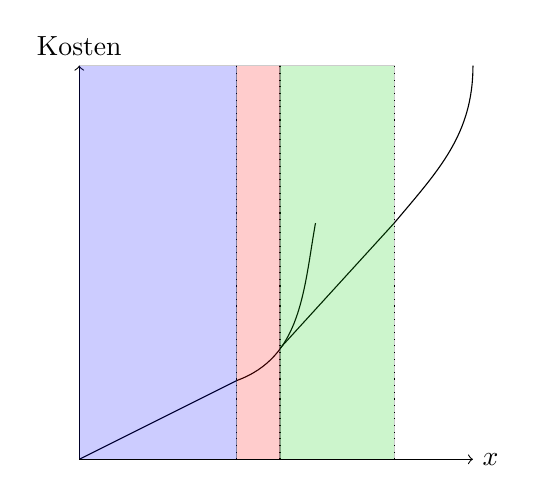
\begin{tikzpicture}
			\draw[->] (0,0) -- (5,0) node[right] {$x$};
			\draw[->] (0,0) -- (0,5) node[above] {Kosten};
			
			\draw (0,0) -- (2,1);
			\draw (2,1) to[out=20,in=-100] (3,3);
			
			\draw (2.55,1.41) -- (4,3);
			\draw (4,3) to[out=50,in=-90] (5,5);
			
			\draw[dotted] (2,0) -- (2,5);
			\draw[dotted] (2.55,0) -- (2.55,5);
			\draw[dotted] (4,0) -- (4,5);
			
			\draw[fill=blue, opacity=0.2] (0,0) rectangle (2,5);
			\draw[fill=red, opacity=0.2] (2,0) rectangle (2.55,5);
			\draw[fill=green!80!black, opacity=0.2] (2.55,0) rectangle (4,5);
			\end{tikzpicture}
		\end{center}
		\begin{center}
			\begin{tabular}{c|ccccccc}
				$x$ & $x_A$ & $x_B$ & $d_A$ & $d_B$ & $t_A$ & $t_B$ & $K(x)$ \\
				\hline
				\textcolor{red}{52} & 0 & 52 & 0 & 5.2 & 0 & 10 & 24772.80 \\
				\textcolor{green!80!black}{60} & 5.6\footnote{$60-x_G$} & 54.4\footnote{$=x_G$} & 4 & 5.44 & 1.4 & 10 & 29848.61
			\end{tabular}
		\end{center}
	\end{enumerate}

	\section*{Aufgabe 6}
	Die zu produzierende Menge liegt im Bereich, wo wir Maschine B\footnote{Maschine B ist billiger, was man daran erkennt, dass die erste Einheit mit ihr erstellt wird.} bis zu $x_G$ voll auslasten und den Rest mit Maschine A produzieren. Wir können ablesen, dass $x_G=94.55$ ist und damit ergibt sich:
	\begin{center}
		\begin{tabular}{c|ccccccc}
			$x$ & $x_A$ & $x_B$ & $d_A$ & $d_B$ & $t_A$ & $t_B$ & $K(x)$ \\
			\hline
			100 & 5.45 & 94.55 & 5 & 9.455 & 1.09 & 10 & 58464.84
		\end{tabular}
	\end{center}
	
\end{document}